\chapter{Perancangan}
\label{perancangan} 

\section{Struktur Proyek Moodle Mobile}
\label{struktur proyek}

Proyek Moodle Mobile terdiri dari kumpulan file-file dan direktori-direktori utama yang mengandung fungsi dan \textit{source code} untuk aplikasi Moodle Mobile, platform Android dan iOS, alat untuk mebangun perangkat lunak, dan konfigurasi. Struktur dapat dilihat di bawah.
\\

\dirtree{%
.1 config.
.1 desktop.
.1 gulp.
.1 hooks.
.1 node\_modules.
.1 platforms.
.1 plugins.
.1 resources. 
.1 scripts.
.1 src.
.2 addon.
.2 app.
.2 assets.
.2 classes.
.2 compontens.
.2 config.json.
.2 configconstants.ts.
.2 core.
.2 directives.
.2 index.html.
.2 lang.
.2 pipes.
.2 providers.
.2 singletons.
.2 theme.
.1 www.
.1 .dockerignore.
.1 .gitattributes.
.1 .gitignore.
.1 .npmrc.
.1 .travis.yml.
.1 config.xml.
.1 Dockerfile.
.1 google-services.json.
.1 gulpfile.js.
.1 ionic.config.json.
.1 LICENSE.
.1 licenses.json.
.1 MainActivity.java.
.1 NOTICE.
.1 packgae-lock.json.
.1 PACKAGE\_PROBLEMS.md.
.1 README.md.
.1 tsconfig.json.
.1 tslint.json.
.1 upgrade.txt.
}

Perubahan pada aplikasi akan sering dilakukan pada direktori \texttt{src}, dan \texttt{config.xml}. Direktori \texttt{src} berisi kode-kode utama dari aplikasi Moodle mobile dan konfigurasinya. Konfigurasi dari Moodle mobile sendiri diatur oleh file \texttt{config.json} di dalam folder \texttt{src}. File \texttt{Config.xml} berfungsi untuk mengatur konfigurasi dari aplikasi Cordova. Dikarenakan Moodle mobile menggunakan Cordova maka pengaturan saat melakukan \textit{build} untuk perangkat bergerak akan diambil dari file \texttt{config.xml}. 

Perubahan juga akan terjadi pada direktori \texttt{resources} dan file \texttt{ionic.config.json}. Direktori \texttt{resource} menyimpan sumber untuk ikon dan \textit{splashscreen} yang akan digunakan oleh aplikasi ketika di-\textit{build} untuk platform Android maupun iOS. File \texttt{ionic.config.json} adalah file konfigurasi yang digunakan oleh  Ionic CLI (\textit{Command Line Interface}), dimana nama aplikasi dan identifikasi aplikasi akan disimpan disana dan dirujuk oleh Ionic CLI ketika digunakan.

Direktori \texttt{node\_modules} juga akan mengalami perubahan namun jarang dilakukan perubahan secara langsung. Dikarenakan direktori tersebut menyimpan \textit{packages} yang dikelola oleh npm. Perubahan yang akan terjadi pada folder \texttt{node\_modules} adalah perubahan seperti yang dibahas di subbab \ref{moodle docs:env}.

\subsection{Perubahan pada \texttt{config.xml}}
Perubahan pada file \texttt{config.xml} akan berpengaruh ketika Cordova membangun aplikasi untuk Android dan iOS karena file \texttt{config.xml} mengatur aturan dan \textit{resource} apa saja yang akan digunakan oleh aplikasi di kedua platform tersebut. 

Perubahan yang dilakukan di dalam file ini adalah sebagai berikut : 

\begin{itemize}
\item Versi aplikasi untuk Android dan iOS akan dimulai dengan versi 1.0.0
\item Nama dari aplikasi adalah \textbf{IDE UNPAR Mobile}
\item Deskripsi aplikasi adalah \textbf{IDE UNPAR app}
\item Penulis aplikasi adalah \textbf{Gabriel Panji Lazuardi} dengan email \textbf{73160068@student.unpar.ac.id}
\item Ikon yang akan digunakan oleh aplikasi dalam platform Android dan iOS.
\item \textit{Splashscreen} yang akan digunakan aplikasi dalam platform Android dan iOS.
\end{itemize}  

\subsection{Perubahan pada direktori \texttt{src}}

Karena direktori ini mengandung \textit{source code} utama dari aplikasi, seluruh perubahan yang bersifat menambah, mengubah ataupun mengahpus fungsi di dalam aplikasi akan terjadi di dalam direktori \texttt{src}. Seluruh fungsi utama aplikasi terletak pada direktori \texttt{src/core}. Untuk pengaturan tema dari aplikasi terletak pada direktori \texttt{src/theme}. Dan folder \texttt{src/app} mengandung \textit{source code} yang akan dijalankan secara \textit{native} pada platform Android dan iOS seperti mengatur warna dari \textit{status bar}.	

Dalam folder \texttt{src/core} setiap fungsi dari Moodle mobile juga dipisah ke dalam direktori masing-masing. Setiap direktori dari fungsi-fungsi tersebut akan memiliki \textit{handler} dan \textit{helper}. \textit{Handler} dari sebuah fungsi bersifat seperti \textit{controller} dari pola desain MVC (\textit{Model-view-controller} perangkat lunak. Sehingga perubahan yang akan dilakukan pada file \textit{handler} adalah perubahan yang bersifat menerima dan memberi data dari dan untuk \textit{view}. Sedangkan \textit{helper} bersifat seperti \textit{model} pada pola desain MVS, sehingga perubahan-perubahan pada \textit{helper} Moodle mobile akan bersifat untuk mengolah dan mengembalikan data.

\section{Menghubungkan IDE UNPAR Mobile dengan Situs IDE UNPAR}
\label{mobile:connect}
Menghubungkan IDE UNPAR mobile dengan situs IDE UNPAR dapat dilakukan dengan melakukan perubahan pada file \texttt{config.json}.  Perubahan yang harus dilakukan adalah menambahkan \textit{key} \textit{"siteurl"} dengan nilai URL yang diinginkan, dalam kasus ini URL yang akan digunakan adalah \url{https://ide.unpar.ac.id}. Dengan adanya \textit{key "siteurl"} aplikasi saaat dijalankan akan langsung melakukan koneksi dengan nilai dari \textit{key} tersebut. Sehingga ketika aplikasi IDE UNPAR Mobile dijalankan, aplikasi akan langsung meminta pengguna \textit{login} dengan tautan \url{https://ide.unpar.ac.id}. Perubahan pada file \texttt{config.json} dapat dilihat pada \mbox{Kode \ref{auto-redirect}}. 

\begin{lstlisting}[language=diff, frame=single, label ={auto-redirect}, caption = Perubahan pada file \texttt{config.json} ]

diff --git a/src/config.json b/src/config.json
index 919869fe652..daaf2aef5c5 100644
--- a/src/config.json
+++ b/src/config.json
@@ -68,10 +68,10 @@
         75.89,
         93.75
     ],
     "demo_sites" :[] ,
     "customurlscheme": "moodlemobile",
-    "siteurl": "https://moodledemo.pascal.id/",
+    "siteurl": "https://ide.unpar.ac.id/",
     "sitename": "",
     "multisitesdisplay": "",
     "sitefindersettings": {},
\end{lstlisting} 

Karena IDE UNPAR menggunakan SSO UNPAR untuk \textit{login} maka aplikasi IDE UNPAR Mobile akan mengarahkan pengguna ke \textit{browser} yang berada pada perangkatnya untuk \textit{login} menggunakan SSO UNPAR. Ketika pengguna telah berhasil \textit{login} agar \textit{browser} pada perangkat pengguna tahu aplikasi apa yang harus dibuka maka \texttt{customurlscheme} pada aplikasi IDE UNPAR Mobile harus diubah. Perubahan untuk \texttt{customurlscheme} dilakukan pada \texttt{config.xml} dapat dilihat di dalam \mbox{Kode \ref{config.xml-scheme}},  \texttt{package.json} dapat dilihat di dalam \mbox{Kode \ref{package.json-scheme}},  dan \texttt{src/config.json} dapat dilihat di dalam \mbox{Kode \ref{config.xml-scheme}}. Dengan perubahan tersebut pengguna akan diarahkan ke dalam aplikasi IDE UNPAR Mobile setelah berhasil \textit{login} menggunakan SSO UNPAR.


\begin{lstlisting}[language=diff, frame=single, label ={config.xml-scheme}, caption = Perubahan pada \texttt{customurlscheme} file \texttt{config.xml} ]

diff --git a/config.xml b/config.xml
index 2e4f35a92ce..67f8cf25744 100644
--- a/config.xml
@@ -648,4 +648,5 @@
             </array>
         </config-file>
     </platform>
+    <variable name="URL_SCHEME" value="idemobile" />
\end{lstlisting} 

\begin{lstlisting}[language=diff, frame=single, label ={package.json-scheme}, caption = Perubahan pada \texttt{customurlscheme} file \texttt{package.json} ]

diff --git a/package.json b/package.json
index a4f73ed0d6d..521d7b943d3 100644
--- a/package.json
+++ b/package.json
@@ -188,7 +189,7 @@
       "cordova-plugin-badge": {},
       "cordova-plugin-camera": {},
       "cordova-plugin-customurlscheme": {
-        "URL_SCHEME": "moodlemobile"
+        "URL_SCHEME": "idemobile"
       },
       "cordova-plugin-device": {},
       "cordova-plugin-file": {},
@@ -255,7 +256,7 @@
       {
         "name": "Moodle Mobile URL",
         "schemes": [
-          "moodlemobile"
+          "idemobile"
         ],
         "role": "Viewer"
       }
\end{lstlisting}

\begin{lstlisting}[language=diff, frame=single, label ={config.json-scheme}, caption = Perubahan pada \texttt{customurlscheme} file \texttt{src/config.json} ]

diff --git a/src/config.json b/src/config.json
index daaf2aef5c5..31402ee6812 100644
--- a/src/config.json
+++ b/src/config.json
@@ -70,7 +70,7 @@
     ],
     "presets" : {"url" :"https://ide.unpar.ac.id/"},
     "demo_sites" :[] ,
-    "customurlscheme": "moodlemobile",
+    "customurlscheme": "idemobile",
     "siteurl": "https://ide.unpar.ac.id/",
     "sitename": "",
     "multisitesdisplay": "",
\end{lstlisting} 

\section{Penerapan Fitur-Fitur Tambahan dari Umpan Balik}

Berdasarkan yang dibahas pada subbab \ref{feature feedback} beberapa saran fitur akan diimplementasikan pada aplikasi IDE UNPAR. Fitur-fitur tersebut adalah PDF \textit{scanner} dan .

\subsection{PDF \textit{scanner}}
\label{feat:pdfscan}
Implementasi fitur ini akan dilakukan dengan bantuan \textit{plugin} Cordova \texttt{cordova-pdf-scanner}. \textit{Plugin} ini dipilih karena memiliki pengaturan paling sederhana. \textit{Plugin} bekerja dengan mengubah HTML mentah ataupun URL menjadi PDF. \textit{Plugin} ini juga dapat mengembalikan hasil pengubahan URL atau HTML mentah ke dalam bentuk base64 agar dapat diunggah kedalam server IDE UNPAR. 

Implementasi fitur PDF \textit{scanner} ini akan dilakukan di direktori \texttt{src/core/fileuploader/}. Dimana \textit{handler} untuk fitur akan disimpan di \texttt{src/core/fileuploader/providers/scanner-handler.ts}. Untuk fungsi memindai gambar untuk diubah menjadi PDF sendiri akan disimpan di \\ \texttt{src/core/fileuploader/providers/helper.ts}. Dengan mengimplementasikan fitur ini pada direktori tersebut, maka fitur ini akan dapat digunakan untuk mengunggah file PDF ke dalam file pribadi pengguna di dalam server IDE UNPAR atau mengungghanya langsung sebagai bentuk submisi tugas atau quiz.\textit{Flow chart} untuk fitur dapat dilihat pada Gambar \ref{fig:scan:flowchart}. 

\begin{figure}[H] 
	\centering  
	\includegraphics[scale=0.6]{FlowChart-ScanPDF.png}  
	\caption[FlowChart untuk fitur PDF \textit{scanner}] {FlowChart untuk fitur PDF \textit{scanner}} 
	\label{fig:scan:flowchart} 
\end{figure} 

File \texttt{src/core/fileuploader/providers/scanner-handler.ts} dapat dilihat pada \mbox{Kode \ref{scanner-handler}}. 

\begin{lstlisting}[language=diff, frame=single, label ={scanner-handler}, caption = File \texttt{scanner-handler.ts} ]

diff --git a/src/core/fileuploader/providers/scanner-handler.ts 
b/src/core/fileuploader/providers/scanner-handler.ts
new file mode 100644
index 0000000000..6cfcbdbc08
--- /dev/null
+++ b/src/core/fileuploader/providers/scanner-handler.ts
@@ -0,0 +1,68 @@
+// (C) Copyright 2015 Moodle Pty Ltd.
+//
+// Licensed under the Apache License, Version 2.0 (the "License");
+// you may not use this file except in compliance with the License.
+// You may obtain a copy of the License at
+//
+//     http://www.apache.org/licenses/LICENSE-2.0
+//
+// Unless required by applicable law or agreed to in writing, software
+// distributed under the License is distributed on an "AS IS" BASIS,
+// WITHOUT WARRANTIES OR CONDITIONS OF ANY KIND, either express or implied.
+// See the License for the specific language governing permissions and
+// limitations under the License.
+
+import { Injectable } from '@angular/core';
+import { CoreAppProvider } from '@providers/app';
+import { CoreUtilsProvider } from '@providers/utils/utils';
+import { CoreFileUploaderHandler, CoreFileUploaderHandlerData } 
  from './delegate';
+import { CoreFileUploaderHelperProvider } from './helper';
+
+@Injectable()
+export class CoreFileUploaderScannerHandler implements 
  CoreFileUploaderHandler {
+    name = 'CoreFileUploaderScanner';
+    priority = 1800;
+
+    constructor(private appProvider: CoreAppProvider, 
+    private utils: CoreUtilsProvider,
+     private uploaderHelper: CoreFileUploaderHelperProvider) { }
+
+    /**
+     * Whether or not the handler is enabled on a site level.
+     *
+     * @return True or promise resolved with true if enabled.
+     */
+    isEnabled(): boolean | Promise<boolean> {
+        return this.appProvider.isMobile() || 
+	this.appProvider.canGetUserMedia();
+    }
+
+    /**
+     * Given a list of mimetypes, return the ones
+     *  that are supported by the handler.
+     * @param mimetypes List of mimetypes.
+     * @return Supported mimetypes.
+     */
+    getSupportedMimetypes(mimetypes: string[]): string[] {
+        return mimetypes;
+    }
+
+    /**
+     * Get the data to display the handler.
+     *
+     * @return Data.
+     */
+    getData(): CoreFileUploaderHandlerData {
+        return {
+            title: 'core.fileuploader.scanner',
+            class: 'core-fileuploader-scanner-handler',
+            icon: 'qr-scanner',
+            action: (maxSize?: number, upload?: 
+	    boolean, allowOffline?: boolean, 
+            mimetypes?: string[]): Promise<any> => {
+                return this.uploaderHelper.scanImage
+	        (maxSize, upload, mimetypes).then((result) => {
+                    return {
+                        treated: true,
+                        result: result
+                    };
+                });
+            }
+        };
+    }
+}
\end{lstlisting} 

Perubahan pada \texttt{src/core/fileuploader/providers/helper.ts} dapat dilihat pada \mbox{Kode \ref{fileuploader-helper}}. 

\begin{lstlisting}[language=diff, frame=single, label ={fileuploader-helper}, caption = Perubahan pada \texttt{src/core/fileuploader/providers/helper.ts} ]
diff --git a/src/core/fileuploader/providers/helper.ts 
b/src/core/fileuploader/providers/helper.ts
index fe28bcb3e4..e69ee619aa 100644
--- a/src/core/fileuploader/providers/helper.ts
+++ b/src/core/fileuploader/providers/helper.ts
+    /**
+     * 
+     * @param maxSize Max size of the upload. -1 for no max size.
+     * @param upload True if file should be uploaded,
+     *  false to return to picked file.
+     * @param mimetypes List of supported mimetypes.  
+     * @return Promise solved when done.
+     */
+    scanImage(maxSize : number,
+    upload?:boolean, mimetypes?: string[]): Promise<any>{
+
+        const camOpts: CameraOptions = {
+            quality: 50,
+            destinationType: this.camera.DestinationType.FILE_URI,
+            correctOrientation: true
+        };
+
+            // Determine the mediaType based on the mimetypes.
+            if (imageSupported && !videoSupported) {
+                camOpts.mediaType = this.camera.MediaType.PICTURE;
+            } else if (!imageSupported && videoSupported) {
+                camOpts.mediaType = this.camera.MediaType.VIDEO;
+            } else if (CoreApp.instance.isIOS()) {
+                // Only get all media in iOS 
+	       //because in Android using this option 
+	      //allows uploading any kind of file.
+                camOpts.mediaType = this.camera.MediaType.ALLMEDIA;
+            }
+        }
+
+        return this.fileUploaderProvider
+	.getPicture(camOpts).then((path) => {
+            const error = this.fileUploaderProvider
+	    .isInvalidMimetype(mimetypes, path); 
+	     // Verify that the mimetype is supported.
+            if (error) {
+                return Promise.reject(error);
+            }
+                const html = '<html> <img src="'+ path +
+	        '" style="width: 100%; height 100%"> </html>';
+                this.logger.debug(html);
+ 	        var currentDate = new Date().getTime();
+                return cordova.plugins.pdf.fromData(html,{
+                    fileName : 'my-pdf'+currentDate,
+                    landscape : "portrait",
+                    type : "base64" 
+		//Using this type because the document 
+		//will be uploaded right away.
+                }).then((base64)=>{   
+                    //converting to blob
+                    const blob = this.base64ToBlob(base64);
+                    
+                    const contentType = 'application/pdf'
+                    const folderPath = "Download/my-pdf"
+ 		+currentDate+".pdf";
+                    return this.fileProvider.writeFile(folderPath, blob)
+		.then((fileEntry)=>{
+                        const options = this.fileUploaderProvider
+			.getFileUploadOptions(fileEntry.nativeURL, +	
+			'mypdf'+currentDate.getTime()+'.pdf',  
+			contentType, true);
+                        if(upload){;
+                            this.logger.debug("uploaded");
+                           return this.uploadFileEntry(fileEntry, true, 
+ 		        -1, upload, false, fileEntry.name);
+                        } else {
+                            // Copy or move the file 
+			to our temporary folder.
+                            this.logger.debug("Copy to temp");
+                            return this.copyToTmpFolder
+ 		         (fileEntry.nativeURL, 
+ 		         false, maxSize, 'pdf', options);
+                        }
+                    
+                    },
+                    (error) => {
+                        this.logger.error(error);
+                    });
+                },(error) => {
+                    const defaultError = 'core.fileuploader
+		.errorcapturingimage';
+                    console.error(error);
+                    return this.treatImageError(error, defaultError);
+                });
+        });
+    
+    }
+
\end{lstlisting}

Setelah melakukan perubahan-perubahan diatas. Fungsi PDF \textit{scanner} akan muncul pada menu aplikasi IDE UNPAR. Namun nama fungsi akan muncul sebagai \texttt{core.fileuploader.scanner} seperti yang terlihat di fungsi \texttt{getData()} pada \mbox{Kode \ref{scanner-handler}}. Untuk mengubah nama fungsi pada menu dierplukan perubahan pada \texttt{src/core/fileuploader/lang/en.json} dan pada \texttt{scripts/langindex.json}. Perubahan-perubahan pada file tersebut dilakukan dengan tujuna agar Moodle mobile dapat mengenali \textit{title} \texttt{core.fileuploader.scanner} dan menterjemahkan ke dalam bahasa yang sesuai.  Perubahan pada \texttt{scripts/langindex.json} dapat dilihat pada \mbox{Kode \ref{langindex.json}} dan perubahan pada \texttt{src/core/fileuploader/lang/en.json} dapat dilihat pada\mbox{Kode \ref{fileuploader-lang-eng}}.

\begin{lstlisting}[language=diff, frame=single, label ={langindex.json}, caption = Perubahan pada file \texttt{langindex.json} ]
diff --git a/scripts/langindex.json b/scripts/langindex.json
index 0a3a21d16d2..2abd385d7a6 100644
--- a/scripts/langindex.json
+++ b/scripts/langindex.json
@@ -1600,6 +1600,7 @@
   "core.fileuploader.uploading": "local_moodlemobileapp",
   "core.fileuploader.uploadingperc": "local_moodlemobileapp",
   "core.fileuploader.video": "local_moodlemobileapp",
+  "core.fileuploader.scanner" : "local_moodlemobileapp",
   "core.filter": "moodle",
   "core.folder": "moodle",
   "core.forcepasswordchangenotice": "moodle",
\end{lstlisting} 

\begin{lstlisting}[language=diff, frame=single, label ={fileuploader-lang-eng}, caption = Perubahan pada file \texttt{src/core/fileuploader/lang/en.json} ]
diff --git a/src/core/fileuploader/lang/en.json
 b/src/core/fileuploader/lang/en.json
index 22d14df4a11..f0b31d17abf 100644
--- a/src/core/fileuploader/lang/en.json
+++ b/src/core/fileuploader/lang/en.json
@@ -25,5 +25,6 @@
     "uploadafile": "Upload a file",
     "uploading": "Uploading",
     "uploadingperc": "Uploading: {{$a}}%",
-    "video": "Video"
+    "video": "Video",
+    "scanner" : "Scan PDF"
 }
\end{lstlisting} 

\subsection{Tautan menuju Student Portal UNPAR}
\label{feat:menu:link}
Seperti yang dibahas pada \ref{absesnsi IDE} akan diimplementasikan sebuah tautan pada menu aplikasi IDE UNPAR yang akan mengarahkan pengguna ke \url{https://studentportal.unpar.ac.id}. Selain menambahkan tautan, pilihan \texttt{change site} pada menu aplikasi akan dihapus karena dirasa pengguna tidak membutuhkan pilihan tersebut.

Perubahan yang harus dilakukan adalah menambahkan sebuah tag HTML \texttt{<a>} yang akan mengarahkan pengguna ke \url{https://sutdentportal.unpar.ac.id} pada \texttt{src/core/mainmenu\\/pages/more/more.html}. Dalam tag HTML \texttt{<a>} tersebut ditambahkan atribut \texttt{(click)} dengan nilai fungsi yang akan dipanggil dari \textit{component} Angular ketika elemen tersebut ditekan. Perubahan pada file \texttt{src/core/mainmenu\\/pages/more/more.html} dapat dilihat pada \mbox{Kode \ref{more-view}}.

\begin{lstlisting}[language=diff, frame=single, label ={more-view}, caption = Perubahan pada file \texttt{src/core/mainmenu/pages/more/more.html} ]
diff --git a/src/core/mainmenu/pages/more/more.html
 b/src/core/mainmenu/pages/more/more.html
index 4b2949e7a04..30c80e2e5d0 100644
--- a/src/core/mainmenu/pages/more/more.html
+++ b/src/core/mainmenu/pages/more/more.html
@@ -39,6 +39,10 @@ <h2>{{ 'core.scanqr' | translate }}</h2>
             <ion-icon name="globe" item-start aria-hidden="true">
	</ion-icon>
             <h2>{{ 'core.mainmenu.website' | translate }}</h2>
         </a>
+        <a *ngIf="showWeb" ion-item (click)="openStudentPortal()" 
+ 	core-link autoLogin="yes" 
+ 	title="{{ 'core.mainmenu.studentportal' | translate }}">
+            <ion-icon name="md-school" item-start aria-hidden="true">
+ 	</ion-icon>
+            <h2>{{ 'core.mainmenu.studentportal' | translate }}</h2>
+        </a>
         <a *ngIf="showHelp" ion-item [href]="docsUrl" 
	core-link autoLogin="no" 
	title="{{ 'core.mainmenu.help' | translate }}">
             <ion-icon name="help-buoy" item-start aria-hidden="true">
	</ion-icon>
             <h2>{{ 'core.mainmenu.help' | translate }}</h2>
@@ -46,10 +50,6 @@ <h2>{{ 'core.mainmenu.help' | translate }}</h2>
         <a ion-item (click)="openSitePreferences()" 
	title="{{ 'core.settings.preferences' | translate }}">
             <core-icon name="fa-wrench" item-start></core-icon>
             <h2>{{ 'core.settings.preferences' | translate }}</h2>
-        </a>
-            <a ion-item (click)="logout()" 
- 	   title="{{ logoutLabel | translate }}">
-            <ion-icon name="log-out" item-start aria-hidden="true">
- 	 </ion-icon>
-            <h2>{{ logoutLabel | translate }}</h2>
         </a>
         <ion-item-divider></ion-item-divider>
         <a ion-item (click)="openAppSettings()" 
	title="{{ 'core.settings.appsettings' | translate }}">
 }
\end{lstlisting} 

Setelah melakukan perubahan pada \texttt{src/core/mainmenu/pages/more/more.html}. Langkah selanjutnya adalah menambahkan fungsi \texttt{openStudentPortal()} pada \texttt{src/core/mainmenu/pages/more/more.ts}. Perubahan dapat dilihat di dalam \mbox{Kode \ref{more-component}}.

\begin{lstlisting}[language=diff, frame=single, label ={more-component}, caption = Perubahan pada file \texttt{src/core/mainmenu/pages/more/more.ts} ]
diff --git a/src/core/mainmenu/pages/more/more.ts
b/src/core/mainmenu/pages/more/more.ts
index a3b786c0717..aa700ff2f08 100644
--- a/src/core/mainmenu/pages/more/more.ts
+++ b/src/core/mainmenu/pages/more/more.ts
@@ -207,4 +207,11 @@ export class CoreMainMenuMorePage implements 
OnDestroy {
     logout(): void {
         this.sitesProvider.logout();
     }
+
+    /**
+     * Open https://studentportal.unpar.ac.id
+     */
+    openStudentPortal() : void{
+        this.utils.openInBrowser( "https://studentportal.unpar.ac.id" );
+    }
 }
\end{lstlisting} 

Menu dengan tautan menuju \url{https://studentportal.unpar.ac.id} sekarang akan muncul, namun dengan nama \texttt{core.mainmenu.studentportal} karena aplikasi tidak mengetahui harus diterjemahkan sebagai kalimat apa. Untuk mengatasi masalah tersebut perlu ditambahkannya \texttt{core.mainmenu.studentportal} di dalam \texttt{src/core/mainmenu/lang/en.json} seperti pada \mbox{Kode \ref{stuper-index}}. Dan menambahkannya juga ke dalam \texttt{scripts/langindex.json} yang ditunjukkan pada  \mbox{Kode \ref{stupor-index-script}}

\begin{lstlisting}[language=diff, frame=single, label ={stupor-index}, caption = Menambahkan \texttt{core.mainmenu.studentportal} pada file  \texttt{src/core/mainmenu/lang/en.json} ]
diff --git a/src/core/mainmenu/lang/en.json 
b/src/core/mainmenu/lang/en.json
index 4ff96fbf7b4..cfbdfb5ac3a 100644
--- a/src/core/mainmenu/lang/en.json
+++ b/src/core/mainmenu/lang/en.json
@@ -2,5 +2,6 @@
     "changesite": "Change site",
     "help": "Help",
     "logout": "Log out",
-    "website": "Website"
+    "website": "Website", 
+    "studentportal": "Student portal UNPAR"
 }
\end{lstlisting} 

\begin{lstlisting}[language=diff, frame=single, label ={stupor-index-script}, caption = Menambahkan \texttt{core.mainmenu.studentportal} pada file  \texttt{scripts/langindex.json} ]
diff --git a/scripts/langindex.json b/scripts/langindex.json
index 2abd385d7a6..e155ef93a01 100644
--- a/scripts/langindex.json
+++ b/scripts/langindex.json
@@ -1862,6 +1862,7 @@
   "core.mainmenu.help": "moodle",
   "core.mainmenu.logout": "moodle",
   "core.mainmenu.website": "local_moodlemobileapp",
+  "core.mainmenu.studentportal" : "local_moodlemobileapp",
   "core.maxfilesize": "moodle",
   "core.maxsizeandattachments": "moodle",
   "core.min": "moodle",
\end{lstlisting} 

\section{Meluncurkan Aplikasi ke dalam Google Play}

Aplikasi akan diluncurkan ke dalam Goog Play yang dikelola oleh FTIS UNPAR. Untuk meluncurkan aplikasi ke dalam Google Play ada beberapa langkah yang harus dilakukan terlebih dahulu. Langkah-langkah tersebut akan dibahas di subsubbab-subsubbab berikut.

\subsection{Membuat apk \textit{release}}

Aplikasi IDE UNPAR Mobile harus dibangun terlebih dahulu dengan pengaturan \textit{production} dan \textit{release}. Membuat \textit{build} dengan pengaturan \textit{release} dapat dilakukan dengan menggunakan perintah \texttt{npx ionic cordova build android --prod --release}. Perintah tersebut akan menghasilkan sebuah apk di \texttt{/moodleapp/platforms/android/app/build/outputs/apk/release} dengan nama \texttt{app-release-unsigned.apk}. Namun, hanya dengan apk tersebut aplikasi tidak akan bisa dimasukkan ke dalam Google Play.

\subsection{Menandai aplikasi secara digital}
Google Play mengharuskan aplikasi yang akan diluncurkan untuk ditandai secara digital. Untuk melakukan hal tersebut diperlukannya sebuah \textit{keystore} yang dapat dibuat dengan \textit{keytool} yang disediakan oleh Java. Membuat \textit{keystore} dengan \textit{keytool} dapat dilakukan dengan perintah \texttt{keytool -genkey -v -keystore idemobile-release-key.keystore -alias ide-unpar-mobile -keyalg RSA \\ -keysize 2048 -validity 100000}, dengan menjalankan perintah tersebut maka sebuah file \textit{keystore} akan dihasilkan dengan nama \texttt{idemobile-release-key.keystore}.

Adanya file \textit{keystore} akan memungkinkan untuk menandai apk \textit{release} yang telah dibuat. Menandai apk dengan file \textit{keystore} dapat dilakukan dengan menggunakan jarsigner yang disediakan oleh Java. Menandai apk dengan jarsigner dilakukan dengan menjalankan perintah \texttt{jarsigner -verbose -sigalg SHA1withRSA -digestalg SHA1 -keystore idemobile-release-key.keystore \\ app-release-unsigned.apk ide-unpar-mobile}. 

\subsection{Finalisasi apk}
Optimasi yang dilakukan adalah menjalankan zipalign kepada apk yang telah ditandai secara digital. Karena pembanguna aplikasi tidak menggunakan Android Studio maka file apk harus di-zipalign secara manual. Zipalign dapat dijalankan dengan perintah \texttt{C:/Users/gabri/AppData/Local/Android/Sdk\\/build-tools/29.0.2/zipalign -v 4 app-release-unsigned.apk ideunparmobile.apk}. Perintah tersebut akan menghasilkan apk yang telah dikompresi dengan nama \texttt{ideunparmobile.apk}. Apk tersebut yang akan diunggah ke dalam Google Play.

\subsection{Mengunggah dan meluncurkan apk}
Apk dari aplikasi IDE UNPAR mobile akan diunggah dengan status \textit{open testing} ke dalam Google Play. Apk akan diunggah melalui Google Play Console. Untuk mengunggha aplikasi dengan status \textit{open testing}, pada menu Google Play Console pilih bagina \textit{Testing} dan kemudian \textit{Open Testing}. Ketika menu tersebut dipilih Google Play Console akan membukakan halaman \textit{Open Testing} seperti pada Gambar \ref{fig:play:open:test}. 

\begin{figure}[H] 
	\centering  
	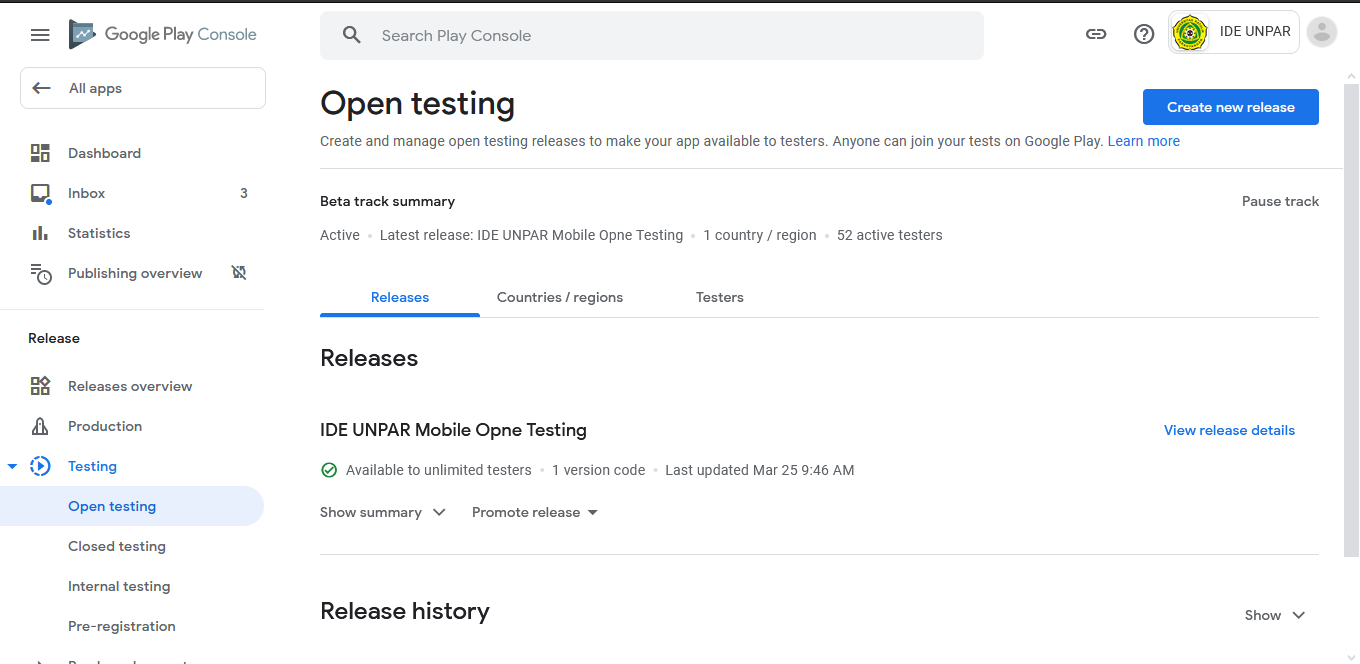
\includegraphics[scale=0.5]{play-console-menu.png}  
	\caption[Halaman \textit{Open Testing}] {Halaman \textit{Open Testing}} 
	\label{fig:play:open:test} 
\end{figure} 

Langkah selanjutnya adalah menekan tombol \textit{Create new release}. Menekan tombol tersebut akan membuka halaman \textit{Create open testing release} sepert pada Gambar \ref{fig:play:open:test:create}. Pada halaman tersebut apk akan diunggah dan detil dari \textit{release} akan diisi.  

\begin{figure}[H] 
	\centering  
	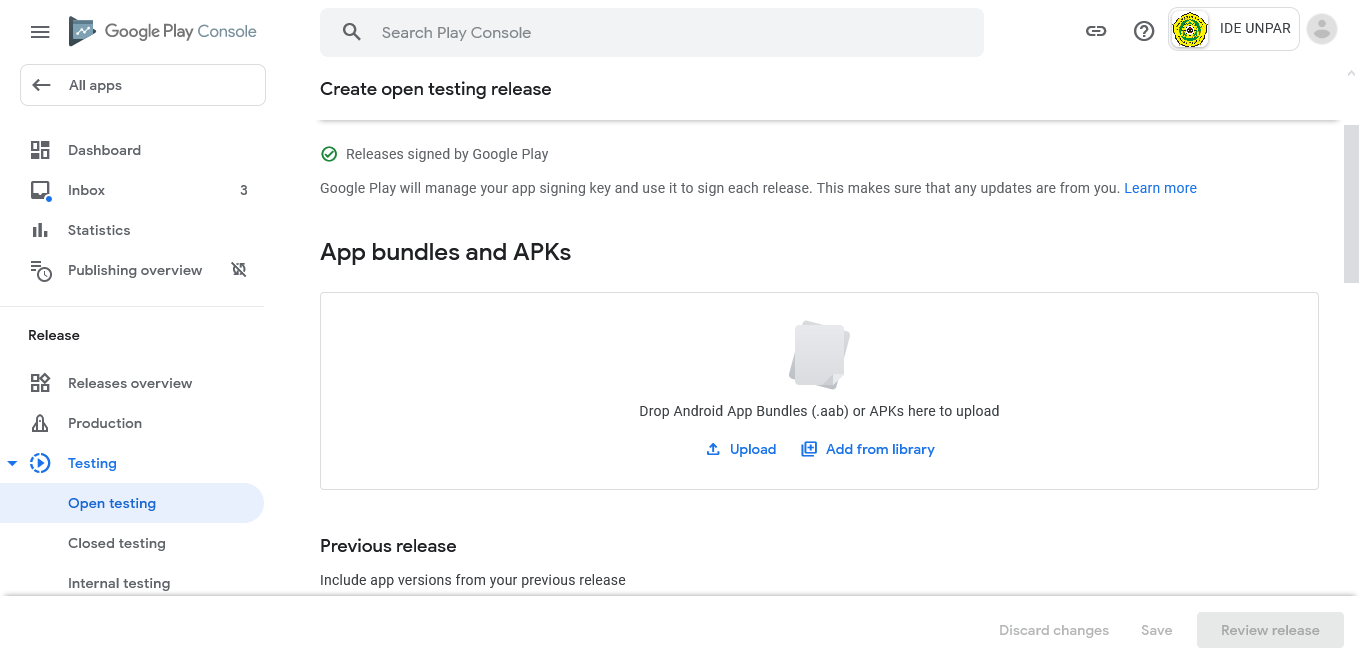
\includegraphics[scale=0.35]{play-create-open-test.png}  
	\caption[Halaman \textit{Create open testing release}] {Halaman \textit{Create open testing release}} 
	\label{fig:play:open:test:create} 
\end{figure} 

Sebelum dapat meluncurkan aplikasi ke dalam Google Play, \textit{release} yang baru saja dibuat harus simpan dan direview terlebih dahulu dengan menekan tombol \textit{Save} kemudian tombol \textit{Review release}. Menekan tombol \textit{Review release} akan membuka halam review seperti pada Gambar \ref{fig:play:open:test:review}. Apabila \textit{release} sudah direview \textit{release} dapat luncurkan dengan menekan tombol \textit{Start rollout to Open testing}.

\begin{figure}[H] 
	\centering  
	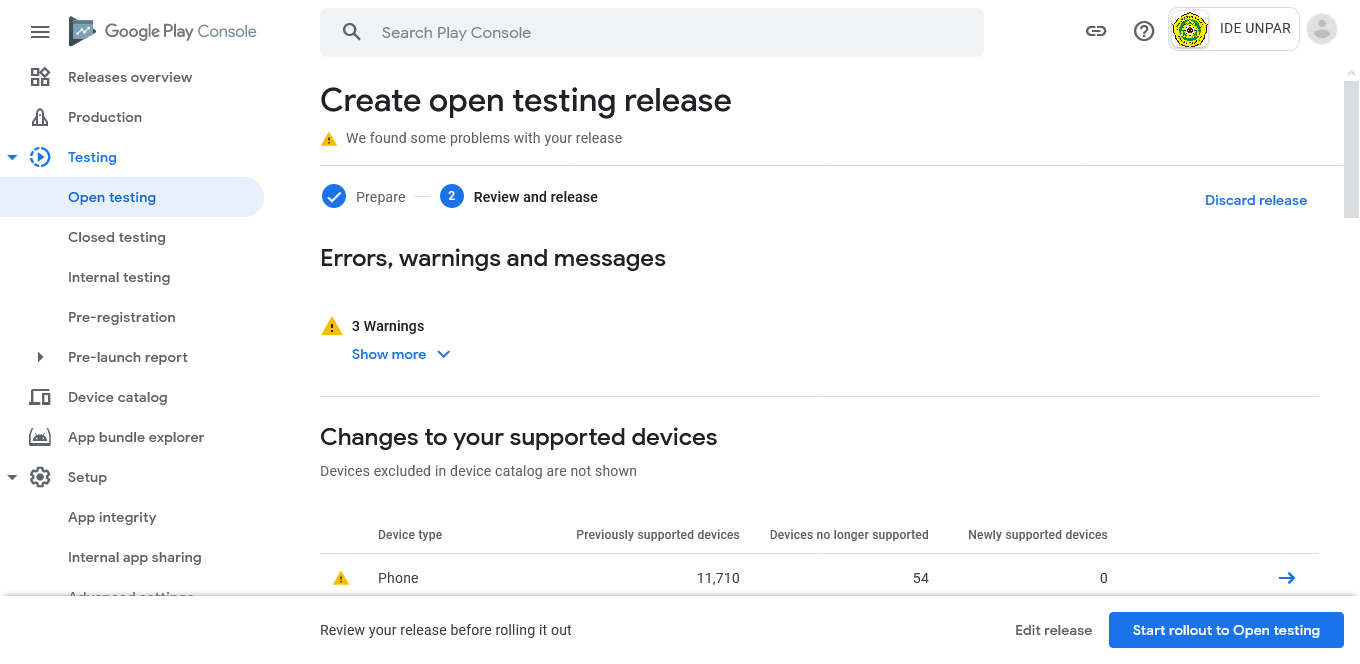
\includegraphics[scale=0.35]{play-review-release.png}  
	\caption[Halaman review \textit{Create open testing release}] {Halaman review \textit{Create open testing release}} 
	\label{fig:play:open:test:review} 
\end{figure} 